% evaluation.tex

We will first mention a few of the general experiences we got doing this project.
We will then discuss the response time results. In Section \ref{eval:throughput} we will discuss the single node throughputs.
Section \ref{eval:balance} discusses the results of the rebalance operations and measured performance scaling. Finally in Section \ref{eval:discussion} we discuss our implementation as a finished product. 

\section{Experiences}

\section{Results discussion}
In this section we will discuss our results and evaluate our system as a whole. We will also briefly discuss issues related to network limits.  

\subsection{Network limits}
We did not have access to different network hardware while doing this project. Our computers proved very capable, with each individual node pushing 34-70 MB per second in raw network data. This made us quickly reach the network speed limit of our gigabit network infrastructure. At this point the load generator was receiving over 130MB/s from the cluster. This limit was reached at around 60k requests per second each of 1024 kB values, providing a hard limit for our throughput. This is why throughput is capped at 60k in our experiments, even though there still are nodes with lots of idle CPU-cycles. On a 100Mbit connection we could only send or receive about 5k requets per second equaling to around 12 MB/s.

\subsection{Network limits}
We did not have access to different network hardware while doing this project. Our computers proved very capable, with each individual node pushing 34-70 MB per second in raw network data. This made us quickly reach the network speed limit of our gigabit network infrastructure. At this point the load generator was receiving over 130MB/s from the cluster. This limit was reached at around 60k requests per second each of 1024 kB values, providing a hard limit for our throughput. This is why throughput is capped at 60k in our experiments, even though there still are nodes with lots of idle CPU-cycles. On a 100Mbit connection we could only send or receive about 5k requets per second equaling to around 12 MB/s

\subsection{Response time distribution and throughput}
\label{eval:responsetime}
In our initial benchmarking experiments we have found no significant difference in the performance when comparing our ZooKeeper implementation with the original Voldemort code. In some cases our implementation is performing slightly better, while in other the opposite is true. We believe this mostly comes down to variance.

Contrary to our expectations, the response time distribution varies greatly on different hardware. In our results the 0.999 percentile response time varies from 250 ms on the slowest hardware to 5 ms on the fastest. On the .90 percentile there is however is much less difference with response times of 2 ms on the slowest hardware and 1 ms on the fastest.

Single-node throughput results are more in line with what we expected. The slow Core 2 Duo is barely able to serve 17k requests per second while the Core i5 and i7 are able to serve 32k and 44k. 

\subsection{Scaling and balancing}
\label{eval:balance}
To achieve full potential scaling some skewing of partitions is required. In our adaptive cluster experiments we have compared automated to manual rebalancing and found our automatic solution to perform on par with the manual one. We have also done a extensive cluster expansion test and monitored CPU-utilization and throughput. These experiments show that our implementation works as intended. 

With optimal partition distribution, a cluster consisting of the two slowest machines was able to service 46k requests per second providing almost the sum of both individual nodes. We also see that a cluster of all three nodes with proper partition distribution easily was able to service the maximum request rate of 60k requests per second. 

\subsection{System evaluation}
\label{eval:discussion}
Overall we are happy with our results. They show that we have not noticeably affected the performance of Voldemort when adding automatic scaling. For now the monitor service is started as a separate process on each node involved in Voldemort. This could be incorporated into Voldemort, but we have not yet done it.  

Our system is best used with diverse clusters of heterogeneous nodes where Headmaster can help automatically partition the dataset across different nodes to improve cluster balance. As the performance loss while rebalancing is not terrible it could be possible to utilize Headmasters rebalancing during peak hours to alleviate struggling nodes. This of course is heavily dependent on partition size. 

Our work should be rather failure tolerant, but as we have not done extensive failure scenario testing, there might still be some bugs. 

We feel that all our goals are met with the system we have created.

\section{General Experiences}

\subsubsection{Server side caching}
While testing, we noticed no real difference between a 12MB and 2GB database cache on our Voldemort servers. This might suggest there is a problem with the cache setting in Voldemort. All of our hardware run on SSDs, but we still consider this result surprising. This could be investigated further using largely different of data sets, but this was not our main focus of this thesis.

\subsubsection{Client updates}
While benchmarking rebalancing we found a critical bug we had introduced in the way clients receive updates of configuration. It caused values being moved during a rebalance to be unavailable for the entire rebalance duration. This would have been hard to discover if we did not compare with the original Voldemort implementation. A graph illustration the issue is available in Figure: \ref{fig:adaptive_bug}

\begin{figure}[h]
    \centering
    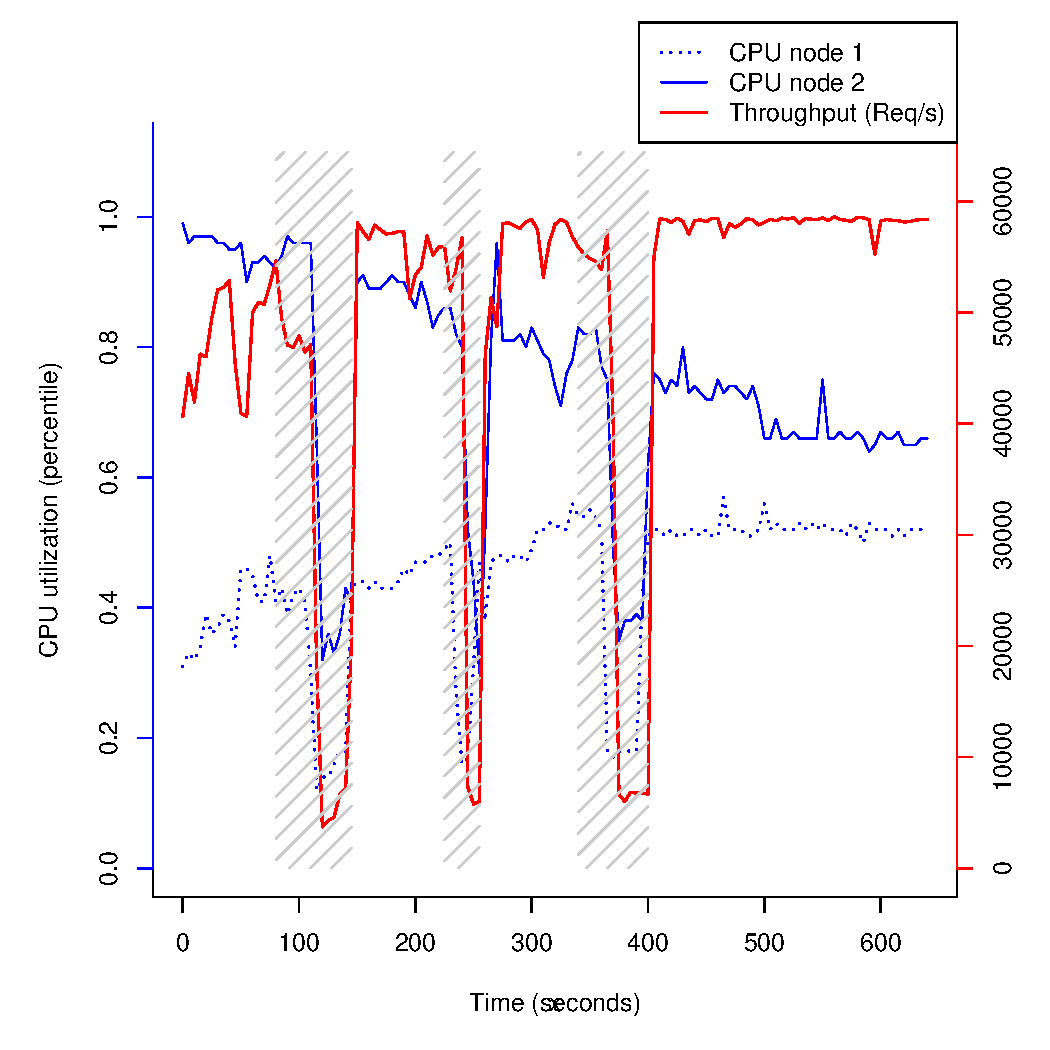
\includegraphics[width=0.7\textwidth]{results/throughput/adaptive/zookeeper/auto_2nodes_error}
    \caption{Fatal bug causing data moved during a rebalance to be inaccessable for close to the entire duration of the rebalance, causing major drops in throughput.}
    \label{fig:adaptive_bug}
\end{figure}

\subsubsection{VectorClock of Stores}
We also had issues with translating a config files version number in ZooKeeper to a valid vector clock in Voldemort. This caused the cluster.xml sent to nodes during a rebalance to be rejected, leading to all proxy-bridges being set up with invalid data. The effect of this bug was that no moved data was accessable during a rebalance. 

\subsubsection{Other notes}
Overall we found the performance to be very consistent. Our results were on large very reproducible and saw little variance between benchmark runs.
